
\chapter{System design}
	\section{System overview} \label{sec:system}

\begin{figure}[h]
    \centering
    \vspace{-0.5cm}
    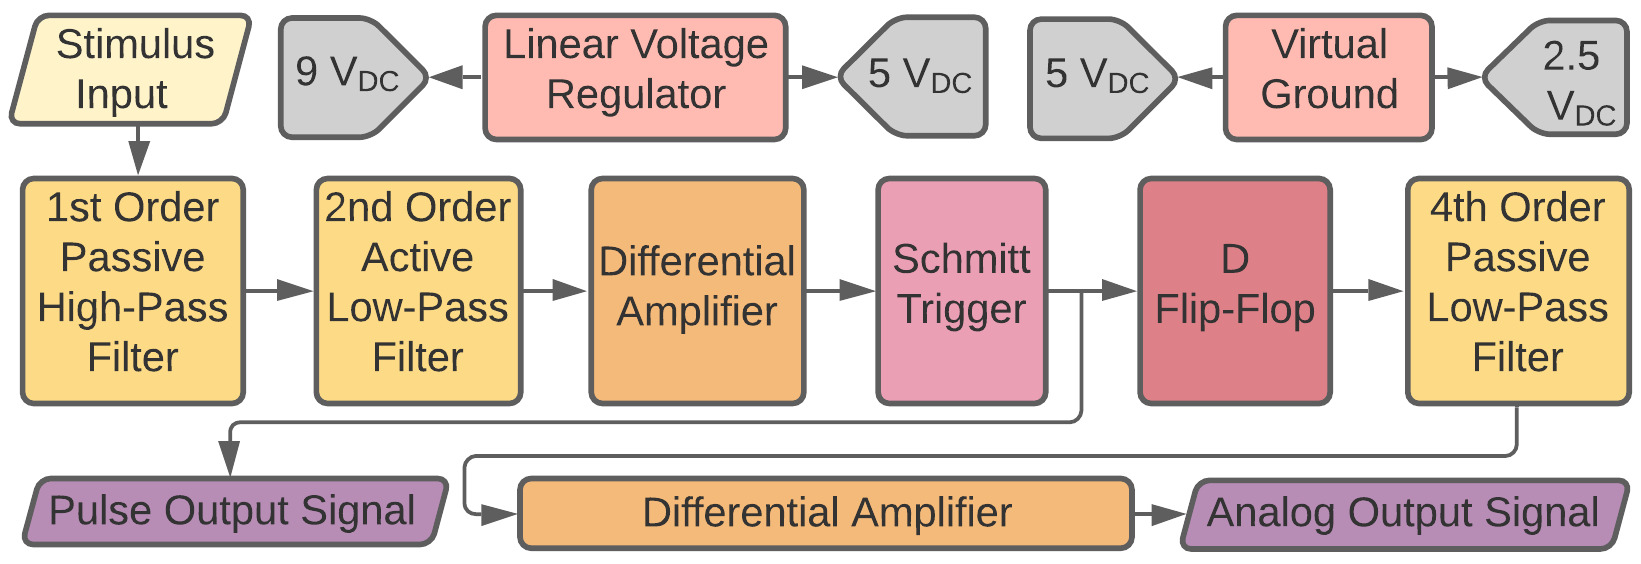
\includegraphics[width = 1\textwidth]{Figures/overview}
    \caption{System Diagram}
    \label{fig:overview}
\end{figure}

A health monitoring system is designed, consisting of a temperature sensor and an optic heart-rate monitor, interacting with a microcontroller. Figure \ref{fig:overview} provides an overview. Since physical sensor measurements are ill-suited for digital interfacing, the main focus of this report is the conditioning, filtering and amplification of the aforementioned.\\

The temperature sensor input is subject to noise, has an unwanted DC offset and an amplitude of insufficient magnitude for AD-conversion. Two second-order low-pass filters were cascaded to clear the signal of noise. This may seem excessive at first, but the cascaded setup allows for the use of less costly components (see Section \ref{sec:temp_design}), as well as producing an output signal subject to very low noise (see Section \ref{sec:temp_results}). Following filtering, amplification is required. Since the filtered signal still contains a DC offset, and the differential amplifier requires a virtual ground, the voltage divider connects to the amplifier in such a way as to simultaneously remove the input DC offset and add the virtual ground. The signal is thus amplified to the degree required by a microcontroller ADC.\\

%Note that this circuit design does not include a voltage buffer, as it was decided against upon noting that the desired output was easily obtained without a buffer, and omitting the buffer resulted in much lower current drawn from the battery (see Appendix C), as well as resulting in lower total cost due to less components present in the circuit. Analysis and simulation of all circuits was done with the simulation software LTSpice.

The heart-rate sensor input is to be converted to a pulse signal and an analogue output, corresponding to heart-beats and the heart-rate respectively. On account of the noise present in the sensor input, signal conditioning  is required. Furthermore, the small amplitude of the sensor input necessitates amplification. A first order passive high-pass filter and a second order active low-pass filter attenuate both high- and low-frequency noise. Despite designing with maximal simplicity in mind to reduce cost and complexity, the filters still performing more than adequately. Thereafter, a differential amplifier produces a signal with a large amplitude and little noise. A Schmitt Trigger then outputs a pulse signal with a frequency corresponding to the heart-rate. The Schmitt Trigger was chosen as it provides a noise margin via hysteresis. An analogue voltage output is required for the microcontroller - filtering and peak detection using diodes was considered but discarded, as non-linear diodes result in extremely slow simulation. Rather, the pulse output signal was converted to a pulse-width modulated signal, where the frequency of the former determines the duty cycle of the latter. This was done as PWM signals lend themselves to conversion-to-analogue by simple filtering. The PWM signal was obtained by using a D Flip-Flop and a RC-circuit \textbf{(see section \ref{sec:heartDesign})}. A fourth order passive RC filter is then used - passive components reduce cost, current usage and simulation time. The filter is of high order as to minimize noise while meeting the settling time requirement. Finally, the signal is amplified to achieve the required range.\\

A microcontroller produces digital readings of the temperature and heart-rate by using the analogue output voltage (representative of the temperature measurement) and the pulse output signal (representing the the heart-rate) in a calibration formula programmed into the microcontroller, where the former is linearly scaled and the latter is converted to a digital reading using the signal frequency. The frequency is detected by measuring the time-interval between rising edges.\\

A voltage regulator supplies power to all sub-circuits of which the system is comprised. Capable of a maximum current of \SI{100}{mA} at \SI{5}{V}, it is more than sufficient to supply the current drawn by Assignments 1, 2 and 3 -  \SI{12.8}{mA}, \SI{13.0}{mA} and \textbf{microcontroller current draw} respectively.

\vfill









